\documentclass[../mathNotesPreamble]{subfiles}
\begin{document}
%  \relscale{1.4}
  \section{6.5: Length of Curves}

  \begin{defn*}[Arc Length for $y=f(x)$]
    Let $f$ have a continuous first derivative on the interval $\sbrkt{a,b}$. The length of the curve from $\parens{a, f(a)}$ to $\parens{b, f(b)}$ is
      \[L=\int_a^b \sqrt{1+f'(x)^2}\,dx.\]
  \end{defn*}

  \vspace*{\stretch{1}}
  \begin{center}
    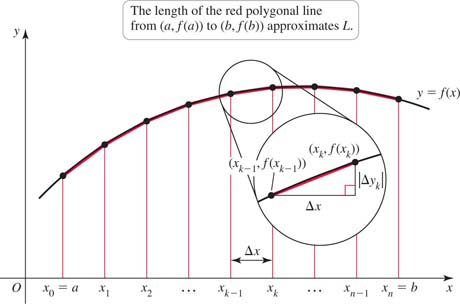
\includegraphics[width=0.6\linewidth]{../images/briggs_06_05/fig06_55}
  \end{center}
  \vspace*{\stretch{1}}
  
  \begin{defn*}[Arc Length for $x=g(y)$]
    Let $g$ have a continuous first derivative on the interval $\sbrkt{c,d}$. The length of the curve from $\parens{g(c),c}$ to $\parens{g(d),d}$ is
      \[L=\int_c^d \sqrt{1+g'(y)^2}\,dy.\]
  \end{defn*}
  \pagebreak

  \begin{ex*}
    Using a geometric argument, we can see that the length of $f(x)=-\dfrac{3}{4}x+\dfrac{7}{2}$ on the interval $\sbrkt{-6,2}$ is $L=10$. Compute this using the arc-length formula.
  \end{ex*}
  \begin{flushright}
    \begin{tikzpicture}
      \begin{axis}[
        grid = both,
        grid style={line width=0.3pt, draw=gray!60},
        axis lines=center,
        axis line style={black,->},
        xmin=-6.75, xmax=3.25,
        ymin=-0.5, ymax=9,
        ymajorticks=false,
        ticklabel style={font=\footnotesize,inner sep=0.5pt,fill=white,opacity=0.5, text opacity=1},
        every axis plot/.append style={line width=0.95pt, color=blue, samples=100},
        width=0.45\linewidth, height=0.3\linewidth
        ]
        \addplot[-, name path=A, ClemsonPurple] expression[domain=-6:2]{-0.75*x+3.5} node[above right, pos=0.3, black, inner sep=0.5pt, opacity=0.75, text opacity=1.0] {$f(x)$};
        \addplot[dashed] (-6,8)--(-6,2)--(2,2);
        \addplot[soldot] coordinates{(-6,8)} node[above right, pos=0.3, black, inner sep=0.5pt, opacity=0.75, text opacity=1.0, font=\normalsize] {$(-6,8)$};
        \addplot[soldot] coordinates{(2,2)} node[above right, pos=0.3, black, inner sep=0.5pt, opacity=0.75, text opacity=1.0, font=\normalsize] {$(2,2)$};
      \end{axis}
    \end{tikzpicture}
  \end{flushright}
  \vspace*{\stretch{1}}
  \pagebreak

  \begin{ex*}
    Find the arc length of the curve $y=\dfrac{1}{4}x^2-\dfrac{1}{2}\ln(x)$, for $1\leq x\leq 2$.
  \end{ex*}
  \vspace*{\stretch{1}}
  \pagebreak

  \begin{ex*}
    Find the arc length of the curve $y=\dfrac{1}{3}x^{\sfrac{3}{2}}$ on $\sbrkt{0,12}$.
  \end{ex*}
  \vspace*{\stretch{1}}
  \pagebreak

  \begin{ex*}
    Find a curve that passes through $\parens{1,2}$ on $\sbrkt{2,6}$ whose arc length is computed using 
      \[\displaystyle \int_2^6 \sqrt{1+16x^{-2}}\,dx.\]
  \end{ex*}
  \vspace*{\stretch{1}}
  
  \begin{ex*}
    Suppose $f$ has length $L$ on $\sbrkt{a,b}$. Evaluate
      \[\int_{\sfrac{a}{c}}^{\sfrac{b}{c}}\sqrt{1+f'(cx)^2}\,dx.\]
  \end{ex*}
  \vspace*{\stretch{1}}
  \pagebreak

\end{document}
